\chapter{Related Work}

\section{Dental caries detection}
Since 2017, there are more than 10 publications regrading automatic caries detection from images \cite{PradosPrivado2020}. They differ in the way, they approach to caries localization as well as in types of images used. The following types of images have been used: Near-Infrared Transillumination images \cite{Casalegno2019,Schwendicke2020}, camera photographs \cite{Moutselos2019} and X-ray images, which may be further divided into bitewing X-ray images \cite{Moran2021, Cantu2020, Bayrakdar2021, Mao2021, Srivastava2017} panoramatic X-ray images \cite{Lian2021} and periapical X-ray images \cite{Lee2018}.

In this chaper we will briefly introduce relevant publications.





\subsection{Manuall detection and classification}
In this section we would briefly introduce publications, that approached caries detection in to following manner: First they crop individual teeth from the X-ray image. Manual cropping or non-machine learning computer vision techniques were used for this purpose. After teeth is extracted from the image, it is labeled by a professional and classifier is trained on this dataset.
\begin{itemize}
    \item First attempts to use a neural network for caries detection date back to 2008, when Kuang et al. \cite{Kuang2008} proposed an approach based on passing a patch from an image to a classifier, which decided if the patch contains caries or healthy enamel. Even though the performance of proposed neural network was surpassed by 6.72\% by kernel SVM, it was still able to outperform an ordinary dentist by more than 5\% and was only 6\% worse than an experienced one
    \item Moran et al.\cite{Moran2021} used methods such as histogram equalization, Otsu's threhsold and morphological operations to extract individual teeth from bitewing images. The dataset was labeled after teeth extraction by assigning one of three categories to each teeth. The categories were: Normal teeth, incipient lesion, advanced lesion. Total of 112 radiographs has been processed this way resulting in 480 teeth with correspoing annotations. ResNet and Inception model was trained to perform the classification task and the best achieved accuracy was 73.3\% \cite{Moran2021}.
    \item{Mao at al. \cite{Mao2021}} did similar preprocessing apprach as Moran, only this time extracting unilateral teeth images insted of the whole teeth. Total of 3716 images of unilateral teeth were obtained. For the purpose of classification AlexNet was used and got 90.3\% accuracy.
    \item{Lee et al. \cite{Lee2018}} published similar approach with periapical images. The dataset with 3000 images was created by manually by cropping out teeth from the X-ray image, keeping only those without bigger dental restorations. By the same process two teeth at once were cropped from the image as well. After obtaining this dataset GoogLeNet and Inception v3 architecure classifiers were trained, obtaining accuracy 89\%  for molars and 82\% for images with both premolars and molars.
\end{itemize}


\subsection{Dental caries segmentation}
There are publications, where the authors approached the task of caries localization as semantic segmentation. Advantage of this approach is pixel precision of the lesion detection. On the other hand creation of similar dataset is very time-consuming. Example of dataset annotated in pixel-wise manner can be seen in figure \ref{fig:segmentation_lit} as well as predictions of a model proposed by Cantu \cite{Cantu2020}.

\begin{figure}
    \centering
    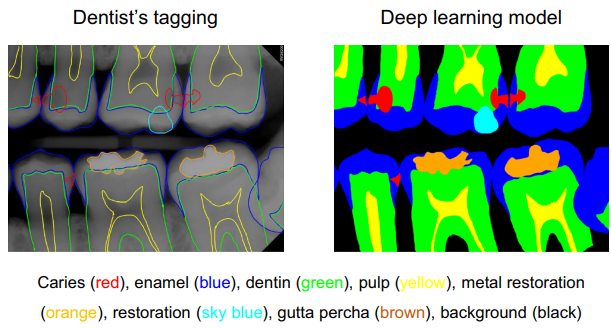
\includegraphics[width=\linewidth]{images/segmentation_bitewing_rich.png}
    \caption{Annotated bitewing radigraph and the same image post-processed, source \cite{Lee2021}}
    \label{fig:bitewing_dense}
\end{figure}

\begin{itemize}
    \item{Cantu et al. \cite{Cantu2020}} created dataset of 3686 bitewing images. In each image, polygonal-shaped box was drawn over caries independently by three dentists. In the case of unanimous decision, the annotation was kept in the datset, otherwise fourth dentist reviewed the annotation and decided if it should be kept or deleted. Cantu et al. used U-net model with EfficientNet B5 as a backbone. The model was evaluated by per pixel and its performance was compared against 7 dentists, outperforming their mean performance in every metric.
    \item{Lian et al. \cite{Lian2021}} had the same apprach as Cantu, but on panoramatic images. In comparison with Cantu, following the segmentation, they cropped region of interest around the segmented lesion and classified the caries into one of four categroies as described in section . They achieved IOU score of 0.785 on the segmentation task. In comparison, the best performing dentist achived IOU of 0.717. In the classification task, the model outperformed the mean dentists performance.
    \item {Lee at al. \cite{Lee2021}} approached the problem in an unique way. In the daset, consisting of 304 bitewing radiographs, they densely annotatated each image by rectagles, not only denoting the position of dental carries, but enamel, denting, pulp, restorations and gutta percha as well. Result of this annotation can be seen in image \ref{fig:bitewing_dense}. They used two independent U-net models to predict position of dental caries and remaining structures in the image. Output of both models was post-processed and merged together. Even though, the model achieved F1-score of 0.641, which is low compoared to other publications. Predictions of the model helped dentists to improve their sensitivity ratio by 7 - 10\%.
\end{itemize}

\begin{figure}
    \centering
    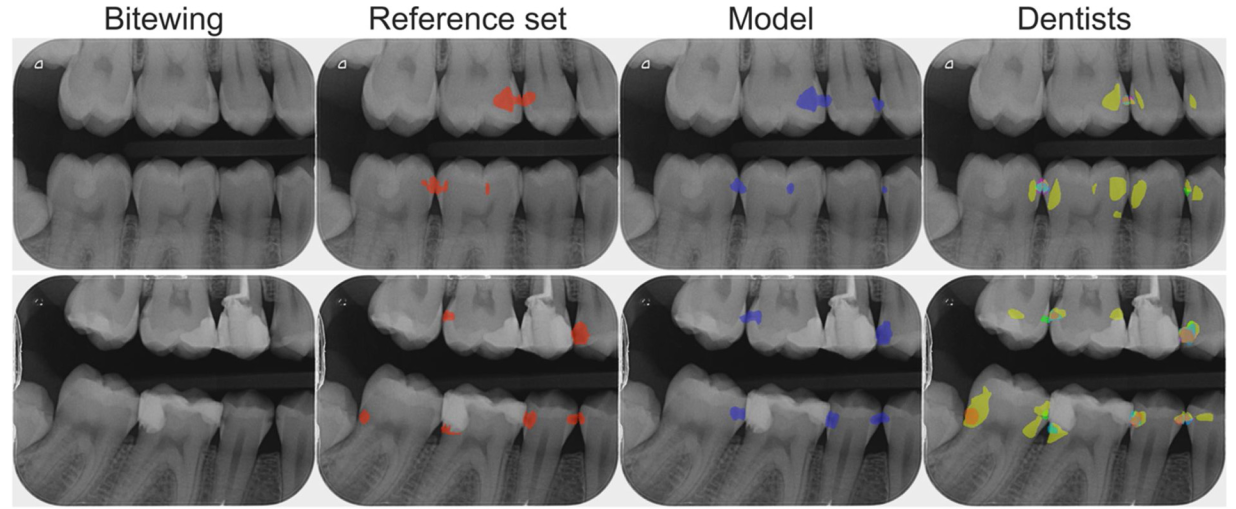
\includegraphics[width=\linewidth]{images/segmentatic_literature.png}
    \caption{Sample of data and predictions of model by }
    \label{fig:segmentation_lit}
\end{figure}

\subsection{Dental caries detection}
\begin{figure}
    \centering
    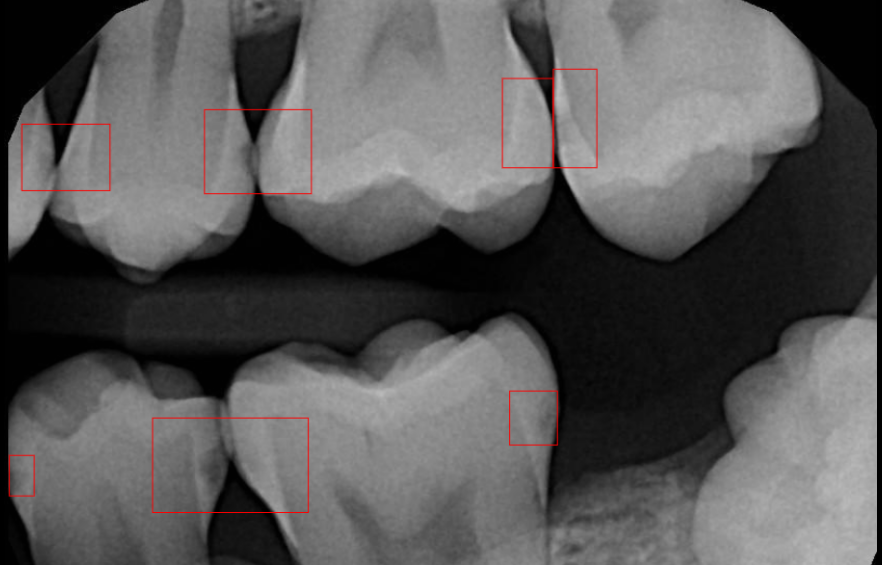
\includegraphics[width=\linewidth]{images/sirvastava_pred.png}
    \caption{Predictions of model proposed by Srivastava et al., source \cite{Srivastava2017}}
    \label{fig:srivastava_preds}
\end{figure}
\begin{itemize}
    \item{Srivastava et al. \cite{Srivastava2017}} trained a fully covolutional neural netowrk with more than 100 layers on a dataset with more than 3000 bitewing radiographs. Position of tooth decay was denoted in pixel-wise manner. Even though the model predicts output masks in semantic segmantation fashion, the output is post-processed by fitting minimal bounding rectangle around the prediction as can be seen in figure \ref{fig:srivastava_preds}. After that the model is evaluated by computing IOU of the rectnagle with ground truth polygon, if the IOU is greater than 0.8, the detection is considered to be positive. Srivastava et al. claims, that their model outerforms by a big margin each of three dentists included in the study. Detailed results are in table \ref{tab:srivastava_results}.

          \begin{table}
              \centering
              \begin{tabular}{c||c|c|c|c|c}
                  Metric    & Model \cite{Srivastava2017} & Model \cite{Kumar2018} & Dr. 1 & Dr. 2 & Dr. 3 \\ \hline
                  Recall    & 0.805                       & 0.70                   & 0.477 & 0.433 & 0.344 \\ \hline
                  Precision & 0.615                       & 0.53                   & 0.63  & 0.815 & 0.891 \\ \hline
                  F1-Score  & 0.70                        & 0.614                  & 0.54  & 0.56  & 0.50
              \end{tabular}
              \caption{Results of models proposed in \cite{Srivastava2017} and \cite{Kumar2018}, compared with three dentists , modified}
              \label{tab:srivastava_results}
          \end{table}

    \item{The same author and Kumar \cite{Kumar2018}} published another paper, where they changed the model to U-Net, which was trained on extended dataset of 6000 bitewing X-ray images. Hard example mining approach was tested by the authors, but led to decrease in performance. Even thought U-Net architecture achieves usually better results on publicly avaliable benchmarks \cite{paperwithcode,Zhang2019} and the size of dataset increased twofold, performance of the model droped by 15\%, see table \ref{tab:srivastava_results}. There are no information available about the evalutation protocol used by Kumar \cite{Kumar2018}, not even about IOU threshold needed to consider a prediction to be correct. This makes it hard to estimate the cause of the performance drop.
    \item{Barakdar et al. \cite{Bayrakdar2021}} did both semantic segmentation and obejct detection. A datset of 621 bitewing images was available for both of those tasks. They claim to use U-net for segmentation and VGGNet for object detection. In the paper it is not mentioned, how te VGGNet architecture for object classification was modified to perform an object detection task. The results of object detection was evaluated aginst 5 professionals in dentistry with different years of experience. The model has outperformed 2 dentists with 2 and 3 yers of experience, while being outperformed by significant margin by all 3 dentists with 10 yers experience. Reported precision of the model is $0.78$, recall=$0.77$ and F1 score of $0.78$. In the paper is no information about the overlap used to consider predictions to be corret. We assume it was set to be $0.5$.
    \item{Bayraktar2021 er al. \cite{Bayraktar2021}} solved only the object detection task on a dataset of 1000 bitewing images labeled by 2 experts with more than 10 years of expreience. With YOLOv3 architecture model, they achieved $AP@.5 = 0.872$ .
\end{itemize}

\section{Dental restorations detection}